\chapter{The crystal oscillator}

In this appendix, the theory of the single-stage transmitter is explained. This is a simple transmitter with one transistor and a crystal. The explanation is divided into multiple parts, starting with the theory of the crystal, followed by the Pierce circuit. Then, we calculate the minimum transconductance needed by the transistor, and finally end with the design of the LC tank circuit and antenna.

Figure~\ref{fig:single_stage_transmitter_circuit} displays the single-stage transmitter circuit, which will be analyzed step by step in the following sections.

This circuit works based on two $180^\circ$ phase shifts of the signal: once by the transistor and once by the crystal. The condition when this phase shift occurs is described below.

\begin{figure}[htbp]
	\centering
	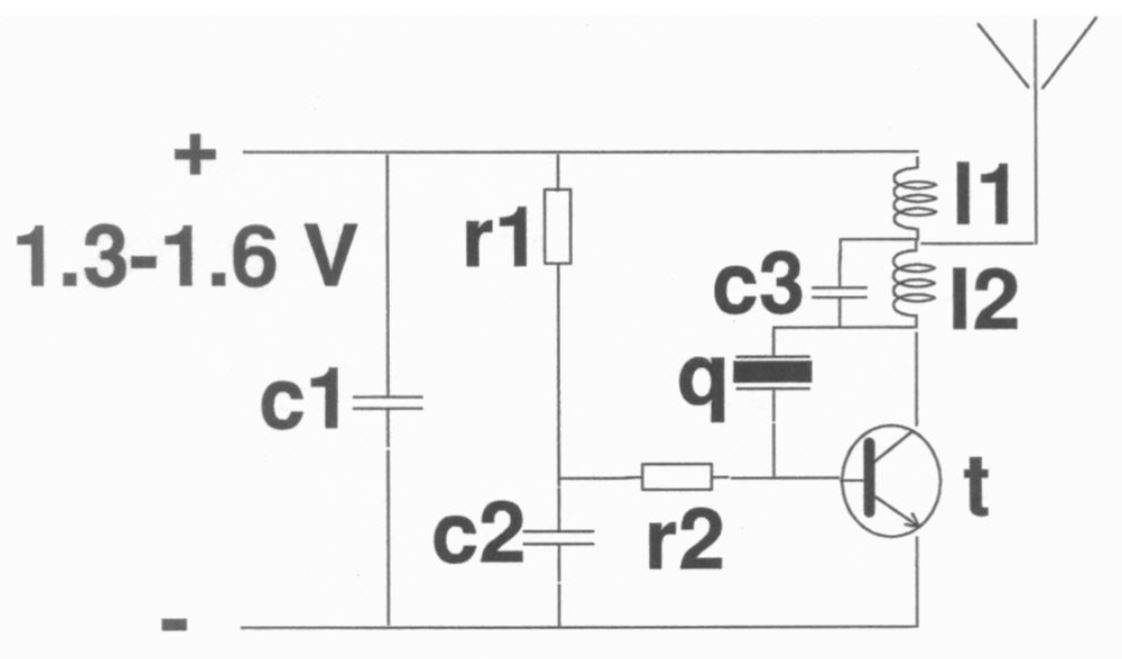
\includegraphics[width=0.75\textwidth]{Single_Stage_Transmitter_Circuit.JPG}
	\caption{Schematic of the single-stage Pierce oscillator circuit (taken from \cite{naef-daenzerNewTransmitterSmall1993a}).}
	\label{fig:single_stage_transmitter_circuit}
\end{figure}

\section{Quartz Crystal}

The quartz crystal sits centrally in the schematic and creates the stable RF signal of the circuit. To achieve the required VHF operating frequency while keeping the crystal physically robust, the crystal is operated in its 3rd overtone mode (approximately three times its fundamental frequency). To analyze its electrical behavior and frequency response, the crystal is represented by the Butterworth-Van Dyke (BVD) equivalent circuit model shown in Figure~\ref{fig:bvd_crystal_equivalent_circuit}.

\begin{figure}[htbp]
	\centering
	\begin{circuitikz}[american, scale=0.85, transform shape]
		% Input terminal
		\draw (0,0) node[left] {A} to[short, o-] (1,0);
		
		% Motional (series) branch: R_s, L_s, C_s
		\draw (1,0) -- (1,1.25)
		to[R, l=$R_s$] (3,1.25)
		to[L, l=$L_s$] (5,1.25)
		to[C, l=$C_s$] (7,1.25) -- (7,0);
		
		% Shunt (parallel) branch: C_0
		\draw (1,0) -- (1,-1.25)
		to[C, l_=$C_0$] (7,-1.25) -- (7,0);
		
		% Output terminal
		\draw (7,0) to[short, -o] (8,0) node[right] {B};
	\end{circuitikz}
	\caption{Butterworth-Van Dyke (BVD) equivalent circuit model of a quartz crystal showing the series motional branch ($R_s, L_s, C_s$) in parallel with the static shunt capacitance ($C_0$) (own work).}
	\label{fig:bvd_crystal_equivalent_circuit}
\end{figure}

The frequency response is derived by combining the series and parallel branches together and determining the resonance conditions.

\begin{equation}
	Z_s(j\omega) = j\omega L_s + \frac{1}{j\omega C_s} = \frac{1 - \omega^2 L_s C_s}{j\omega C_s}, \quad Z_0(j\omega) = \frac{1}{j\omega C_0}
\end{equation}

Combining both equations in parallel yields:

\begin{align}
	Z(j\omega) &= Z_s(j\omega) \parallel Z_0(j\omega) \nonumber \\
	&= \frac{\left(\frac{1 - \omega^2 L_s C_s}{j\omega C_s}\right) \cdot \left(\frac{1}{j\omega C_0}\right)}{\left(\frac{1 - \omega^2 L_s C_s}{j\omega C_s}\right) + \frac{1}{j\omega C_0}} \nonumber \\
	&= \frac{1 - \omega^2 L_s C_s}{j\omega \left[ (C_s + C_0) - \omega^2 L_s C_s C_0 \right]} \nonumber \\
	&= \frac{1}{j\omega C_0} \cdot \frac{\frac{1}{L_s C_s} - \omega^2}{\frac{1}{L_s}\left(\frac{1}{C_s} + \frac{1}{C_0}\right) - \omega^2}
\end{align}

Finding the zeros and poles of $Z(j\omega)$ shows the resonant frequencies of the quartz crystal:

\begin{enumerate}
	\item \textbf{Series Resonant Frequency ($f_s$):} Occurs when $Z(j\omega) = 0$:
	\begin{equation}
		f_s = \frac{1}{2\pi \sqrt{L_s C_s}}
	\end{equation}
	\item \textbf{Parallel Resonant Frequency ($f_p$):} Occurs when $Z(j\omega) \to \infty$. Factoring out $C_s$ directly relates $f_p$ to $f_s$:
	\begin{equation}
		f_p = \frac{1}{2\pi} \sqrt{\frac{1}{L_s C_s} \left(1 + \frac{C_s}{C_0}\right)} = f_s \sqrt{1 + \frac{C_s}{C_0}}
	\end{equation}
\end{enumerate}

Since $C_0 \gg C_s$, the ratio $\frac{C_s}{C_0} \ll 1$. Applying a first-order Taylor series approximation ($(1 + x)^{1/2} \approx 1 + \frac{x}{2}$) provides a simplified expression for the parallel resonant frequency:

\begin{equation}
	f_p \approx f_s \left(1 + \frac{C_s}{2 C_0}\right)
\end{equation}

For $f < f_s$ and $f > f_p$, the circuit behaves like a capacitor, whereas for $f_s < f < f_p$, it behaves like an inductor. These properties will be important when defining the oscillation conditions in the Pierce circuit.


\section{Pierce oscillator}

The Pierce oscillator works on the basis that a quartz crystal and two capacitors will induce a $180^\circ$ phase shift onto a signal. Inverting that signal then results in an oscillation following the Barkhausen criteria, meaning the total phase shift must be $k \cdot 360^\circ$ ($k \in \mathbb{N}$) and the amplification should be $\ge 1$.

\begin{figure}[htbp]
	\centering
	\begin{circuitikz}[american, scale=1.1, transform shape]
		% Top Branch: Inverter U1
		\draw (0,3) node[circ] {} -- (0.8,3)
		node[not gate US, draw, anchor=input] (ng) {}
		(ng.output) -- (3.5,3) node[circ] {} to[short, -o] (4.2,3);
		\node[above=2pt] at (ng.north) {$U_1$};
		
		% Middle-Upper Branch: Resistor R1
		\draw (0,1.8) node[circ] {} to[R, l=$R_1$] (3.5,1.8) node[circ] {};
		
		% Middle-Lower Branch: Quartz Crystal X1
		\draw (0,0.5) node[circ] {} to[piezoelectric, l=$Q_1$] (3.5,0.5) node[circ] {};
		
		% Vertical Connecting Rails
		\draw (0,3) -- (0,0.5);
		\draw (3.5,3) -- (3.5,0.5);
		
		% Bottom Left: Capacitor C1 to Ground
		\draw (0,0.5) to[C, l_=$C_C$] (0,-1) to[ground] (0,-1.3);
		
		% Bottom Right: Capacitor C2 to Ground
		\draw (3.5,0.5) to[C, l=$C_B$] (3.5,-1) to[ground] (3.5,-1.3);
	\end{circuitikz}
	\caption{A Pierce oscillator circuit.}
	\label{fig:pierce_inverter_gate_circuit}
\end{figure}

In the following steps, $C_b$ and $C_c$ represent the total node capacitances from base to ground and collector to ground, respectively. The feedback resistor and inverter are removed in this analysis, as the transistor functions as the inverting element.

We start by modeling the collector-to-base voltage ratio using a voltage divider formed by the crystal reactance $X_q$ and the base capacitance $C_b$:

\begin{equation}
	Z_b(j\omega) = \frac{1}{j\omega C_b}, \quad Z_q(j\omega) = j X_q
\end{equation}

Applying the voltage divider rule yields the base voltage $V_b$ relative to the collector voltage $V_c$:

\begin{align}
	\frac{V_b}{V_c} &= \frac{Z_b(j\omega)}{Z_q(j\omega) + Z_b(j\omega)} \nonumber \\
	&= \frac{\frac{1}{j\omega C_b}}{j X_q + \frac{1}{j\omega C_b}} \nonumber \\
	&= \frac{1}{1 - \omega C_b X_q}
\end{align}

To achieve the required $180^\circ$ phase shift, the transfer ratio must be negative ($\frac{V_b}{V_c} < 0$). This requires the denominator $1 - \omega C_b X_q$ to be negative. Since $\omega$ and $C_b$ are strictly positive, $X_q$ must be positive ($X_q > 0$), confirming that the crystal must operate in its inductive reactance region ($f_s < f < f_p$).

An important effect of the node capacitances $C_b$ and $C_c$ is that they alter the resonant frequency of the quartz crystal, which must be taken into account. Looking from the crystal terminals, $C_b$ and $C_c$ are in series with each other and in parallel with $C_0$. The total external load capacitance $C_L$ experienced by the crystal is defined as:

\begin{equation}
	C_L = \frac{C_b C_c}{C_b + C_c}
\end{equation}

In addition to the static capacitance $C_0$ and the external load capacitance $C_L$, the internal transistor feedback capacitance $C_\mu$ (between collector and base) also sits directly in parallel across the crystal terminals. Combining these contributions yields the total effective parallel capacitance $C_T$:

\begin{equation}
	C_T = C_0 + C_L + C_\mu = C_0 + \frac{C_b C_c}{C_b + C_c} + C_\mu
\end{equation}

Consequently, the loaded parallel resonant frequency $f_p$ expressed in terms of $C_T$ becomes:

\begin{equation}
	f_p = f_s \sqrt{1 + \frac{C_s}{C_T}}
\end{equation}

Applying the first-order Taylor approximation ($(1+x)^{1/2} \approx 1 + \frac{x}{2}$) yields the simplified expression for the loaded frequency:

\begin{equation}
	f_p \approx f_s \left(1 + \frac{C_s}{2 C_T}\right)
\end{equation}


\section{Transconductance calculation}

In this section, the critical transconductance ($g_{m,\text{crit}}$) of the transistor is derived to determine the threshold condition for oscillation startup. This is done by deriving the negative resistance generated by the BJT and adjusting for losses inside the quartz crystal.

\begin{figure}[htbp]
	\centering
	\begin{circuitikz}[american, scale=1.0, transform shape]
		% Base (B) and Collector (C) Nodes
		\draw (0,2) node[circ] {} node[left] {$B$} node[above=8pt, right=4pt] {$V_b$}
		(6,2) node[circ] {} node[right] {$C$};
		
		% Ground Rail
		\draw (-0.5,0) -- (6.5,0);
		\draw (3,0) node[ground] {};
		
		% Left Branch: Base Small-Signal Network (R2 // Cb)
		\draw (0,2) to[R, l_=$R_2$] (0,0);
		\draw (0,2) -- (1.5,2);
		\draw (1.5,2) to[C, l=$C_b$] (1.5,0);
		
		% Miller capacitance C_mu between Base and Collector (replaces former short)
		\draw (1.5,2) node[circ] {} to[C, l=$C_\mu$, label distance=0pt] (4.5,2) node[circ] {};
		
		% Right Branch: BJT Transconductor (gm*Vb) & Collector Capacitance (Cc)
		\draw (4.5,2) to[isource, l_=$g_m V_b$] (4.5,0);
		\draw (4.5,2) -- (6,2);
		\draw (6,2) to[C, l=$C_c$] (6,0);
		
		% Top Branch: Butterworth-Van Dyke (BVD) Crystal Model across B and C
		\draw (0,2) -- (0,5);
		\draw (6,2) -- (6,5);
		
		% Static Capacitance C0 Branch
		\draw (0,3.3) node[circ] {} to[C, l=$C_0$] (6,3.3) node[circ] {};
		
		% Motional Series Branch (Rs - Ls - Cs)
		\draw (0,4.8) node[circ] {} 
		to[R, l=$R_s$] (2,4.8) 
		to[L, l=$L_s$] (4,4.8) 
		to[C, l=$C_s$] (6,4.8) node[circ] {};
		
		% Red current arrow indicating current flowing OUT of the crystal and INTO the collector
		\draw[->, >=latex, red, thick] (6,3.1) -- (6,2.2) node[midway, left] {$i_q$};
	\end{circuitikz}
	\caption{Small-signal equivalent circuit of the BJT Pierce oscillator with current $i_q$ flowing from the crystal feedback network into the collector node.}
	\label{fig:bjt_pierce_small_signal_model}
\end{figure}

\subsubsection*{Node B Analysis}
The bias resistor $R_2$ can be neglected assuming it is sufficiently large.

\begin{equation}
	V_b = -\frac{i_q}{j\omega C_b}
\end{equation}

\subsubsection*{Node C Analysis (KCL)}
Applying KCL at Node C, the sum of currents entering the node equals the sum of currents leaving to ground.

\begin{equation}
	i_q = g_m V_b + j\omega C_c V_c
\end{equation}

Solving for $V_c$ directly from the Node C:

\begin{equation}
	V_c = \frac{i_q - g_m V_b}{j\omega C_c}
\end{equation}

Substituting $V_b$ into this expression gives:

\begin{align}
	V_c &= \frac{i_q - g_m \left(-\frac{i_q}{j\omega C_b}\right)}{j\omega C_c} \nonumber \\
	&= \frac{i_q}{j\omega C_c} - \frac{g_m i_q}{\omega^2 C_b C_c}
\end{align}

Combining these two nodes with $i_q$ results into the impedance seen by the quartz crystal.

\begin{align}
	V_c - V_b &= \left( \frac{i_q}{j\omega C_c} - \frac{g_m i_q}{\omega^2 C_b C_c} \right) - \left( -\frac{i_q}{j\omega C_b} \right) \nonumber \\
	&= i_q \left( \frac{1}{j\omega C_b} + \frac{1}{j\omega C_c} - \frac{g_m}{\omega^2 C_b C_c} \right) \nonumber \\
	&= i_q \left( -\frac{g_m}{\omega^2 C_b C_c} - j \frac{C_b + C_c}{\omega C_b C_c} \right)
\end{align}

Dividing by $i_q$ defines the active transistor input impedance $Z_t$ seen by the crystal:

\begin{equation}
	Z_t = \frac{V_c - V_b}{i_q} = -\frac{g_m}{\omega^2 C_b C_c} - \frac{j}{\omega C_L}
\end{equation}

where $C_L = \frac{C_b C_c}{C_b + C_c}$ is the equivalent series load capacitance. The negative real part $R_a = -\frac{g_m}{\omega^2 C_b C_c}$ provides the active power necessary to overcome system losses and initiate oscillation.

\subsubsection*{Power Balance and Critical Transconductance}

To determine the startup threshold condition, the crystal current $i$ is modeled as dividing between two parallel branches across the terminal voltage $v$:

\begin{itemize}
	\item \textbf{Branch A (Active Circuit):} Impedance $Z_t = R_a - \frac{j}{\omega C_L}$
	\item \textbf{Branch P (Parasitics):} Combined capacitance $C_p = C_0 + C_\mu$, with impedance $Z_p = \frac{1}{j\omega C_p}$
\end{itemize}

Applying Kirchhoff's Current Law (KCL) at the node and expressing the currents using branch admittances ($Y = \frac{1}{Z}$):

\begin{equation}
	i = i_a + i_p
\end{equation}

\begin{equation}
	v = i_a Z_t = i_p Z_p \implies i_a = v Y_t, \quad i_p = v Y_p
\end{equation}

Summing the branch currents allows $v$ to be expressed in terms of the total current $i$:

\begin{equation}
	i = v(Y_t + Y_p) \implies v = \frac{i}{Y_t + Y_p}
\end{equation}

Substituting $v$ back into the active branch current $i_a = v Y_t$ gives the exact current divider equation:

\begin{equation}
	i_a = i \frac{Y_t}{Y_t + Y_p}
\end{equation}

The branch admittances are defined as $Y_p = j\omega C_p$ and $Y_t = \frac{1}{R_a - j/(\omega C_L)}$. Assuming $|R_a| \ll \frac{1}{\omega C_L}$, the active impedance is dominated by its capacitive term ($Z_t \approx -\frac{j}{\omega C_L}$), simplifying the active admittance to $Y_t \approx j\omega C_L$.

Substituting $Y_t$ and $Y_p$ back into the current divider yields:

\begin{align}
	i_a &= i \frac{j\omega C_L}{j\omega C_L + j\omega C_p} \nonumber \\
	&= i \frac{C_L}{C_L + C_p} \nonumber \\
	&= i \frac{C_L}{C_L + C_0 + C_\mu} = i \frac{C_L}{C_T}
\end{align}

where $C_T = C_L + C_0 + C_\mu$ represents the total parallel capacitance.

Real power is exchanged solely within the active resistance $R_a$ (driven by $i_a$) and the crystal's series loss resistance $R_s$ (driven by $i$):

\begin{equation}
	P_{\text{supplied}} = |R_a| i_a^2 = |R_a| \left(\frac{C_L}{C_T}\right)^2 i^2
\end{equation}

\begin{equation}
	P_{\text{loss}} = R_s i^2
\end{equation}

Equating $P_{\text{supplied}} = P_{\text{loss}}$ and canceling $i^2$:

\begin{equation}
	R_s = |R_a| \left(\frac{C_L}{C_T}\right)^2
\end{equation}

Substituting $|R_a| = \frac{g_m}{\omega^2 C_b C_c}$ yields the final critical transconductance $g_{m,\text{crit}}$ required for oscillation startup:

\begin{equation}
	g_{m,\text{crit}} = \omega^2 C_b C_c R_s \left(\frac{C_T}{C_L}\right)^2
\end{equation}


The resulting $g_{m,\text{crit}}$ is used to calculate the required base bias current. To ensure a reliable startup, it is recommended to maintain a design margin of $g_m = (3 \text{ to } 5) \times g_{m,\text{crit}}$.

The DC collector bias current $I_c$ is determined from the transconductance $g_m$ and the thermal voltage $V_T$:

\begin{equation}
	I_c = g_m V_T
\end{equation}

where $V_T = \frac{k_B T}{q} \approx 25.85\text{ mV}$ at room temperature ($300\text{ K}$).

The corresponding base bias current $I_b$ is obtained using the transistor's common-emitter current gain $\beta$:

\begin{equation}
	I_b = \frac{I_c}{\beta} = \frac{g_m V_T}{\beta}
\end{equation}

Keep in mind that $V_T$ and $\beta$ fluctuate with temperature and operating conditions, so extreme values should be taken into account when creating a practical design.


\section{Collector arm}

The Pierce oscillator requires a capacitive reactance on both sides of the quartz crystal. On the collector side, this capacitance is named $C_c$, but in reality, it consists of a network comprising two inductors, a capacitor, and an antenna. For the oscillator to operate, this network must have a net capacitive reactance at the oscillation frequency.

\begin{figure}[htbp]
	\centering
	\begin{circuitikz}[american, scale=1.0, transform shape]
		% Collector Terminal C
		\draw (0,2) node[circ] {} node[left] {$C$};
		
		% Parallel Tank Network (L2 // C3) between Node C and Node J
		\draw (0,2) -- (0,3) to[L, l=$L_2$] (3,3) -- (3,2);
		\draw (0,2) -- (0,1) to[C, l_=$C_3$] (3,1) -- (3,2);
		
		% Junction Node J
		\draw (3,2) node[circ] {} node[left=2pt] {$J$};
		
		% Inductor L1 Branch to Ground
		\draw (3,2) -- (4.5,2) node[circ] {};
		\draw (4.5,2) to[L, l=$L_1$] (4.5,0) node[ground] {};
		
		% Antenna Series Load Branch (Ca + R_rad) to Ground
		\draw (4.5,2) -- (6.5,2);
		\draw (6.5,2) to[C, l=$C_a$] (6.5,0.8) 
		to[R, l=$R_{\text{rad}}$] (6.5,-0.5) node[ground] {};
		
		% Antenna Label
		\node[right] at (6.8, 0.15) [right=20pt]{(Antenna)};
	\end{circuitikz}
	\caption{Equivalent circuit representation of the collector network connected to the parallel $L_2//C_3$ tank, $L_1$ matching inductor, and the antenna load model ($C_a, R_{\text{rad}}$).}
	\label{fig:collector_antenna_matching_network}
\end{figure}

The lower bound of the capacitive frequency range for the collector arm is defined by $\omega_{\text{tank}} = \frac{1}{\sqrt{L_2 C_3}}$, where $L_1 \parallel C_a$ is simplified to $L_1' = \frac{L_1}{1 - \omega^2 L_1 C_a}$.

The upper bound is obtained by requiring a net capacitive reactance:

\begin{equation}
	\omega L_1' + \frac{\omega L_2}{1 - \omega^2 L_2 C_3} < 0
\end{equation}

Dividing by $\omega > 0$ and multiplying by $(1 - \omega^2 L_2 C_3) < 0$ (which reverses the inequality sign since $\omega > \omega_{\text{tank}}$) yields:

\begin{align}
	L_2 &> -L_1' \left(1 - \omega^2 L_2 C_3\right) \nonumber \\
	L_1' + L_2 &> \omega^2 L_1' L_2 C_3 \nonumber \\
	\omega^2 &< \frac{1}{L_2 C_3} \left(1 + \frac{L_2}{L_1'}\right)
\end{align}

Substituting $\omega_{\text{tank}}^2 = \frac{1}{L_2 C_3}$ defines the valid frequency range for capacitive collector behavior:

\begin{equation}
	\omega_{\text{tank}} < \omega_{\text{osc}} < \omega_{\text{tank}} \sqrt{1 + \frac{L_2}{L_1'}}
\end{equation}

The tank circuit must be designed such that the oscillation frequency falls within these frequency bounds.

\section{The antenna}
